%%
%% Copyright 2007, 2008, 2009 Elsevier Ltd
%%
%% This file is part of the 'Elsarticle Bundle'.
%% ---------------------------------------------

%% Please read the file, ``Addtional_AuthorInstruction_LaTeX.pdf'', for choosing the following options. 
%% Please choose only one of the two following options. Note that the option \final, which is also provided below, must not be submitted.
%\def\preprint{1}			% Use for submitted manuscript
\def\wordcount {1}		% Use for word count

%% The following option provides the final print version. This is only for personal use. Don't use this for submission.
%\def\final {1}

%% Please do not modify the following nine lines
\ifdefined\preprint
  \documentclass[preprint,review,12pt]{elsarticle}
\fi
\ifdefined\wordcount
  \documentclass[final,3p,times,twocolumn]{elsarticle}
\fi
\ifdefined\final
  \documentclass[final,3p,times,twocolumn]{elsarticle}
\fi

%% Graphics packages for PostScript figures
%%\usepackage{graphics}
\usepackage{graphicx,stfloats}
\usepackage{color}
\usepackage{graphicx}
%% Other useful packages
%\usepackage{latexsym}
%\usepackage{subfigure}
\usepackage{caption}
\usepackage{subcaption}
\usepackage{float}
\usepackage{multirow}
\usepackage{threeparttable}
%% The amssymb package provides various useful mathematical symbols
\usepackage{amssymb}
\usepackage{amsmath}
\usepackage{siunitx}
\usepackage{subfiles}
%% The amsthm package provides extended theorem environments
%\usepackage{amsthm}
%\usepackage{hyperref}
%\hypersetup{colorlinks = true}

%\definecolor{CeruleanRef}{RGB}{12,127,172}
%\captionsetup[figure]{name={Fig.},labelsep=period}
%\renewcommand{\figureautorefname}{Fig.}
%\def\equationautorefname~#1\null{Eq.~(#1)\null}

\biboptions{sort&compress}

\journal{Proceedings of the Combustion Institute}

\begin{document}

\begin{frontmatter}

\title{Sensetivity Analysis}

\author{Ahmed Hassan\corref{cor1}}
\ead{a.hassan@itv.rwth-aachen.de}
\author{Moataz Sabry}
\author{Vincent Le Chenadec}
\author{Taraneh Sayadi}



\address{Institute for Combustion Technology, RWTH Aachen University, 52064 Aachen, Germany}
%\address[sec]{Second affiliation, Address, City and Postcode, Country}
\cortext[cor1]{Corresponding author.}

\begin{abstract}

Adjoint sensitivity analysis of ignition delay time for a zero-dimension reactor is presented in this work. A developed work package based on the algorithmic differentiation technique is used to provide accurate jacobins. The numerical jacobians provided by algorithmic differentiation are similarly accurate as analytical ones encounter the approximated derivatives using finite difference schemes. The framework is extendable for different configurations without extra effort. The proposed approach provides a superior accurate and robust computational method for the sensitivity of any parameter contribute to the governing equations ( Arrhenius, thermodynamic, etc.).          

\end{abstract}

\begin{keyword}

Sensitivity analysis \sep Uncertainty quantification \sep Enthalpy of formation \sep Standard entropy \sep Heat capacity

\end{keyword}

\end{frontmatter}

\clearpage

\section{Introduction}
\label{Introduction}

TBD
\section{Primal problem}
The governing equations that describe an ideal homogeneous  zero-dimensional isochoric reactor are as follows,
\begin{equation}
\frac{\partial Y_i}{\partial t}=\frac{1}{\rho}\dot{\omega}_i
\end{equation}
\begin{equation}
\frac{\partial T}{\partial t}=\frac{1}{\rho C_v}\dot{\omega''}_T
\end{equation}

where $Y_i$, is the species mass fraction vector $i=[1, ........, N]	$, $C_v$, $\rho$ are the heat capacity at constant volume, the density respectively, $\dot{\omega}_i$ is the rate of consumption or production for the different species and  $\dot{\omega"}_T$ is the heat released rate which is defined by,

\begin{equation}
\label{eq:EST}
\dot{\omega"}_T=-\sum_{i=1}^{N} \dot{\omega}_i u_i,
\end{equation} 
knowing that $u_i$ is the total internal and chemical energy and driven from the enthalpy,
\begin{equation}
u_i=h_i-R T.
\end{equation} 
The reaction rate of different species $i$ due to the set of reactions $N_r$ is expressed as, 
\begin{equation}
\label{eq:SST}
\dot{\omega}_i=\sum_{j=1}^{N_r} \dot{\omega}_{ij}.
\end{equation}     
The consumption/production rate of species based on each reaction is $\dot{\omega}_{ij}= q_j {M}_i {\nu}_{ij} $ where $M_i$ is the molecular weight of species $i$, $ {\nu}_{ij}$ is the stoichiometric molar balance between reactants and products of species $i$ involves in reaction$j$,$ {\nu}_{ij}= {\nu''}_{ij}- {\nu'}_{ij}$. The reaction rates $q_j$ are modelled as follow,
 
 \begin{equation}
 q_j={k_f}_j \prod_{i=1}^{N}[X_i]^{{\nu'}_{ij}}-{k_r}_j \prod_{i=1}^{N}[X_i]^{{\nu''}_{ij}},
 \end{equation}

where the forward and reverse reaction rate constants of reaction $j$ are ${k_f}_j$ and ${k_r}_j$ respectively, and the molar concentration of species $i$ is $[X_i]$. The thermodynamic quantities are computed based on NASA polynomial empirical model {\color{red} add ref}. The ideal gas equation $p=\frac{\rho R T}{\bar{M}}$ is used to close the system, as $\bar{M}$ is the average molecular weight and $R $ is the universal gas constant. 
\subsection{reaction rates models}
The forward rate coefficients are generally computed using Arrhenius parameters. Depending on how the forward rate constants change with the pressure, additional reaction types, such as three-body and uni-molecular/recombination fall-off reactions, are also considered. Lindemann and Troe forms are used to express the rate constants of pressure-dependent fall-off reactions.The reverse rate constants are related to the forward rate constants through the equilibrium constants or through own Arrhenius parameter in case explicitly mentioned in the mechanism data. 


\subsection{Mechanisms}
\subsubsection{H2/O2}
The first scheme under consideration is the hydrogen oxidation mechanism described by Ó Conaire et al. [29]. It includes 40 reactions among 10 species consisting of 5 elements, i.e. O, H, C, N, and Ar.

\subsubsection{GRI 3.0}
The second examined scheme is the well-known gri3.0 [30] reaction scheme. The model includes 325 reactions and 53 species.
\section{Methodology}
\label{Methodology}
The most common method in sensitivity analysis is based on the gradient descendant technique for continuous, differentiable, and convex functions {\color{red} add ref}, and this is also the case for our model.
 As there are several approaches to compute the gradients (brute force, Forward sensitivity, and Adjoint, etc.), and each one has its advantages and disadvantages, a detailed comparison is provided in  {\color{red} add ref}. The adjoint approach scales with the number of the objective functions/quantity of interests(QOI) independent of the system parameters number based on that the adjoint approach was chosen{\color{red} add ref}.  
\subsection{Forward solution}
The forward solution of the primal problem  are split into two main steps reading the chemical mechanism files including thermodynamic properties and set up the numerical framework    	

\subsection{Adjoint approach}
There are several adjoint approaches as fully continuous, fully discrete, and semi discrete{\color{red} add ref}.  The studied system is zero-dimensional so only fully continuous/discrete techniques are applicable. for this study, the fully continuous method is considered. The general derivation of  adjoint equations for system of non linear coupled ordinary differential equations(ODE) as follow, 
consider an objective function of multiple imputes and single outputs, $y=J(q_i,g_j)$, where$y \rightarrow R$ as $q_i \rightarrow R^n$, $g_j \rightarrow R^m$ are the state vector and system parameters( thermodynamic, Arrhenius ,etc.) respectively. The objective function could represent any quantity of interest (QoI) produced by the system like ignition delay time or average temperature etc. The Lagrangian function is used to remove the dependencies between the state variables and system parameters, 
\begin{equation}
\mathcal{L}(q_i,\textbf{g})=J-\mathbf{\lambda} \cdot \int_{0}^{t_f} (\frac{\partial q_i}{\partial t}- F(q_i\textbf{g}))dt-a_i\cdot (q_i-q_0)\big|_{t=0},
\end{equation}    
where $\lambda$ and $a$ are the lagrangian variables vectors , $F(q_i,\textbf{g})$ are the governing equations right hand side and $(q_i-q_0)\big|_{t=0}$ are the initial conditions, taking the derivative of $\mathcal{L}(q_i,\textbf{g})$ with respect to $q_i$ leads to the following adjoint equations.
\begin{equation}
\frac{\partial \mathcal{L}(q_i,\textbf{g})}{\partial q_i} \delta q_i=\frac{\partial J}{\partial q_i} \delta q_i-\lambda_i\int_{}^{} \frac{\partial \delta{q_i}}{\partial t}-\frac{\partial F(q_i,\textbf{g})}{\partial q_i}\delta q_i dt-a_i \delta q_i\big|_{t=0}, 
\end{equation}
applying integration by parts to the above equation,
\begin{equation}
\frac{\partial \mathcal{L}(q_i,\textbf{g})}{\partial q_i} \delta q_i=\frac{\partial J}{\partial q_i} \delta q_i+\delta{q_i}\int_{}^{} \frac{\partial \lambda_i}{\partial t}+\lambda_j \frac{\partial F_j}{\partial q_i}dt-a_i \delta q_i\big|_{t=0}-\lambda_i \delta q_i\big|_{t=0}^{t_f}, 
\end{equation}
in case $J$ is an integral QoI  then it can be expressed as $J=\int_{}^{} h dt $ and by substituting in the above equation
\begin{equation}
\frac{\partial \mathcal{L}(q_i,\textbf{g})}{\partial q_i} \delta q_i=\delta{q_i}\int_{}^{} \frac{\partial h}{\partial q_i}+\frac{\partial \lambda_i}{\partial t}+\lambda_j\frac{\partial F_j}{\partial q_i}dt-a_i \delta q_i\big|_{t=0}-\lambda_i \delta q_i\big|_{t=0}^{t_f}, 
\end{equation}

then by cancelling the perturbation $\delta q_i$ the adjoin equation is as follow,
\begin{equation}
0=\frac{\partial h}{\partial q_i}+\frac{\partial \lambda_i}{\partial t}+\lambda_j \frac{\partial F_j}{\partial q_i}.
\end{equation}
Eliminating the perturbation $\delta q_i$ at $t=0$ and $
t=t_f$, as the values of $\lambda_i$ are known at $t=t_f$, this imposes an initial conditions for the above equations $\lambda_i=0\Big|_{t=t_f}$, due to these initial conditions the adjoint equations are integrated backward in time, which requires a very dense mesh to achieve high accuracy {\color{red} add ref}.
%Fully discrete adjoint enforces using a self adjoint time integrator or derive the adjoint form of the preferred time integrator, the first option is not applicable as highly non-linear ODEs solved using  high order Range-kouta(RK) schemes which are not self adjont, and deriving there adjoint version is out of this study scope. Fully contionous adjoint 



Computing the jacobians for highly non-linear systems requires checking pointing that is stored during the forward solution of the primal problem, because of the asynchronous between the forward and the backward time integration. A high-order interpolation function is used to overcome the fidelity difference. 
\subsection{Computing derivatives}

There are several methods to compute the derivatives that construct the jacobians, one of the most common techniques is the Fréchet derivative {\color{red} add ref}. Although it is easy to implement, this method is error-prone which is accurate depending on the proposed perturbation value similar to the FD method. Complex step differentiation (CSD) prevents the loss of precision inherited in the traditional finite difference, however, still not so accurate and on top of that, the main disadvantage is the high computational time consumption for both of the methods. These disadvantages make FD and CSD are out of scope, especially for large systems. To achieve high accuracy affordably a working package based on algorithmic differentiation (AD) method is coded up from scratch in Julia Language likewise the governing equations~\ref{eq: GE}. The new AD tool provides the values of reaction rates and the thermodynamic quantities, and their gradients with respect to all system variables and parameters% involved  
%in the source term of species and energy equations ~\ref{eq:SST}~\ref{eq:EST} 
fast and as accurate as analytical derivatives. It is important to note that, Julia is a new programming language made for facilitating the computation of scientific applications. Julia combines execution speed on a par with statistically-typed languages with the active performance provided by dynamic languages  {\color{red} add ref}.
      
%\subsection{Algorithmic differentiation}
\subsection{Sensitivity analysis of ignition delay time}
\label{SensitivityAnalysis}
The ignition process involves a sudden increase in the temperature accompanies by changes in the species profiles. The variation in the behaviour of the species profile changes according to the mechanism used in the modelled reactor, so it is hard to put a general and identical description to ignition based on the specific field. But globally the rapid increase in the temperature distinguishes the ignition phenomenon independent of the applied mechanism so that the phase shift in the temperature profile could mimic the ignition delay time {\color{red} add ref} and the QOI is written as follow
\begin{equation}
J=\frac{1}{\tau}\int_{}^{} (T-T^{shift})^2dt.
\end{equation}
The transitioned profile $T^{shift}$  is determined from the relation $T^{shift}(t)=T(t-10^{-2}\cdot t_r)$, where $t_r$ is the characteristic time of ignition and computed based on the maximum time gradient for temperature $\frac{dT}{dt}\Big|_{max}$ leading to the equation
\begin{equation}
tr=\frac{T_{max}-T_0}{\frac{dT}{dt}\Big|_{max}}.
\end{equation} 
Figure~\ref{fig:figure1} visualizes the difference between the original and the delayed profile, showing a schematic vision to the value of $t_r$.  

\begin{figure}
\centering
 {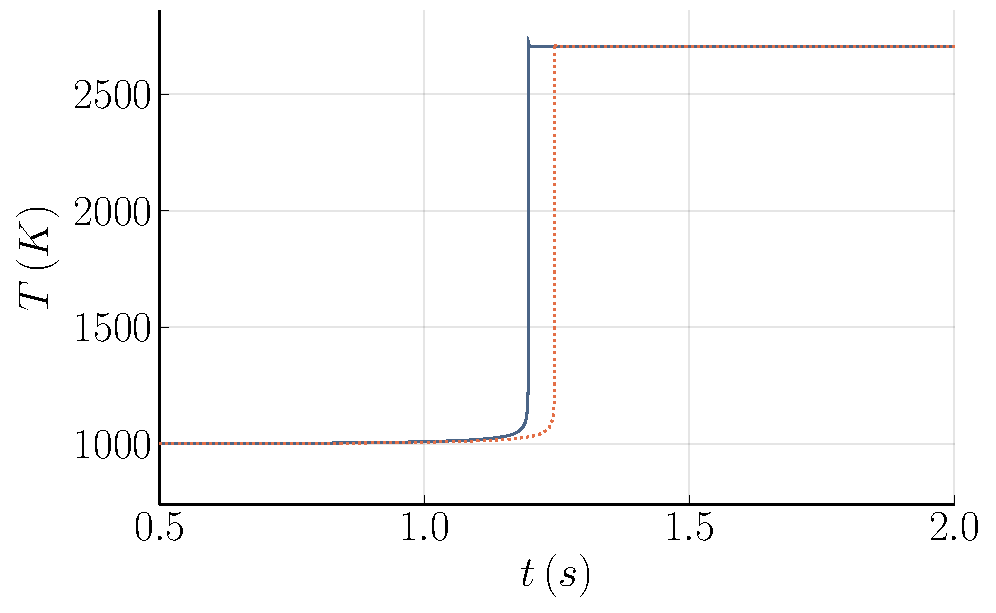
\includegraphics[width=0.5\textwidth]{figures/time shift without legend.pdf}}
\caption{comparison between the reference temperature profile.-----, shifted profile;  {\color{red} .....}   }
    \label{fig:figure1}
 \end{figure}
The gradients of the QOI with respect to system parameter $\frac{d J}{dg_i}$ is derived from the Lagrangian function {\color{red} add ref}  as follow 
%\begin{equation}
%\frac{\partial \mathcal{L}(g_i,\textbf{q})}{\partial g_i} \delta g_i=\delta{g_i}\int_{}^{} \frac{\partial h}{\partial g_i}+\lambda_j\frac{\partial F_j}{\partial g_i}dt, 
%\end{equation}
% as $\frac{d J}{dg_i}=\frac{\partial \mathcal{L}(g_i,\textbf{q})}{\partial g_i} $ then the grad
\begin{equation}
\frac{d J}{dg_i}= \int_{}^{} \frac{\partial h}{\partial g_i}+\lambda_j\frac{\partial F_j}{\partial g_i}dt.
\end{equation}
Finally, the sensitivity is normalized and related to $\frac{d J}{dg_i}$ as follow  {\color{red} add ref}, 
\begin{equation}
S_i=\frac{g_i}{J}\cdot\frac{d J}{dg_i}
\end{equation}   



\section{Results and Validation}
The first step is validating the primal problem~\ref{GE} implementation in the newly developed AD tool  {\color{red} name of the tool}. For the sake of validation the $gri3.0$ mechanism is simulated by Cantera and Flame Master {\color{red} add ref} with initial mass fractions of $Y_{CH_4} = 0.05$ and $Y_{O_2} = 0.2$ and $N_2=0.75$, as initial temperature $T=1000 K$ at atmospheric pressure condition is used and compared to the results of {\color{red} name of the tool}. The perfect matching between temperature and species profiles obtained by different software as shown in figure~\ref{fig:figure2} and figure \ref{fig:figure3} insures the veracity of the simulation of the governing equations by {\color{red} name of the tool}.

      \begin{figure}
\centering
 {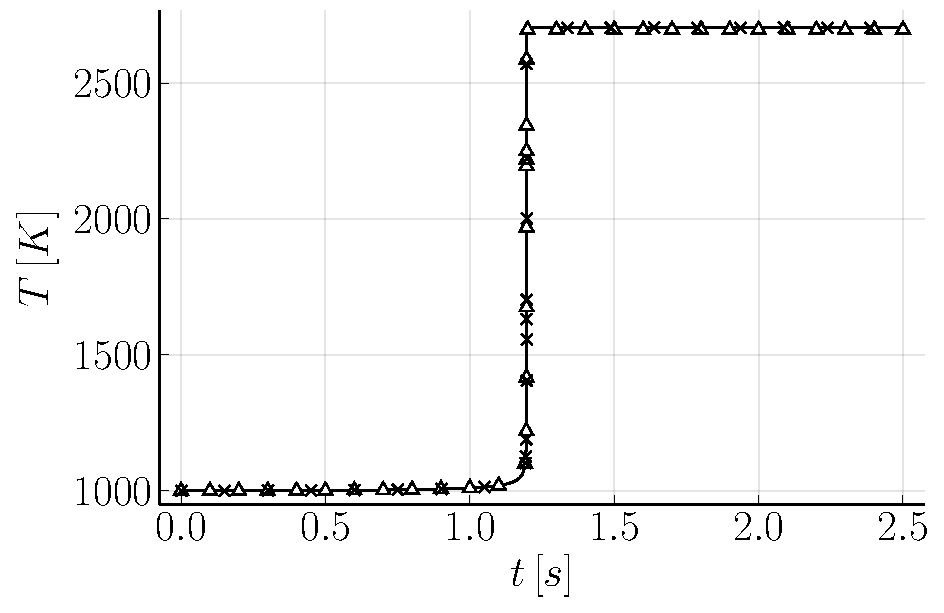
\includegraphics[width=0.5\textwidth]{figures/T validation.pdf}}
\caption{comparison between the temperature profile obtained by different software .-----, AD tool; x, Cantera; $\Delta$, Flame Master  }
    \label{fig:figure2}
 \end{figure}   
 \begin{figure}
\centering
 {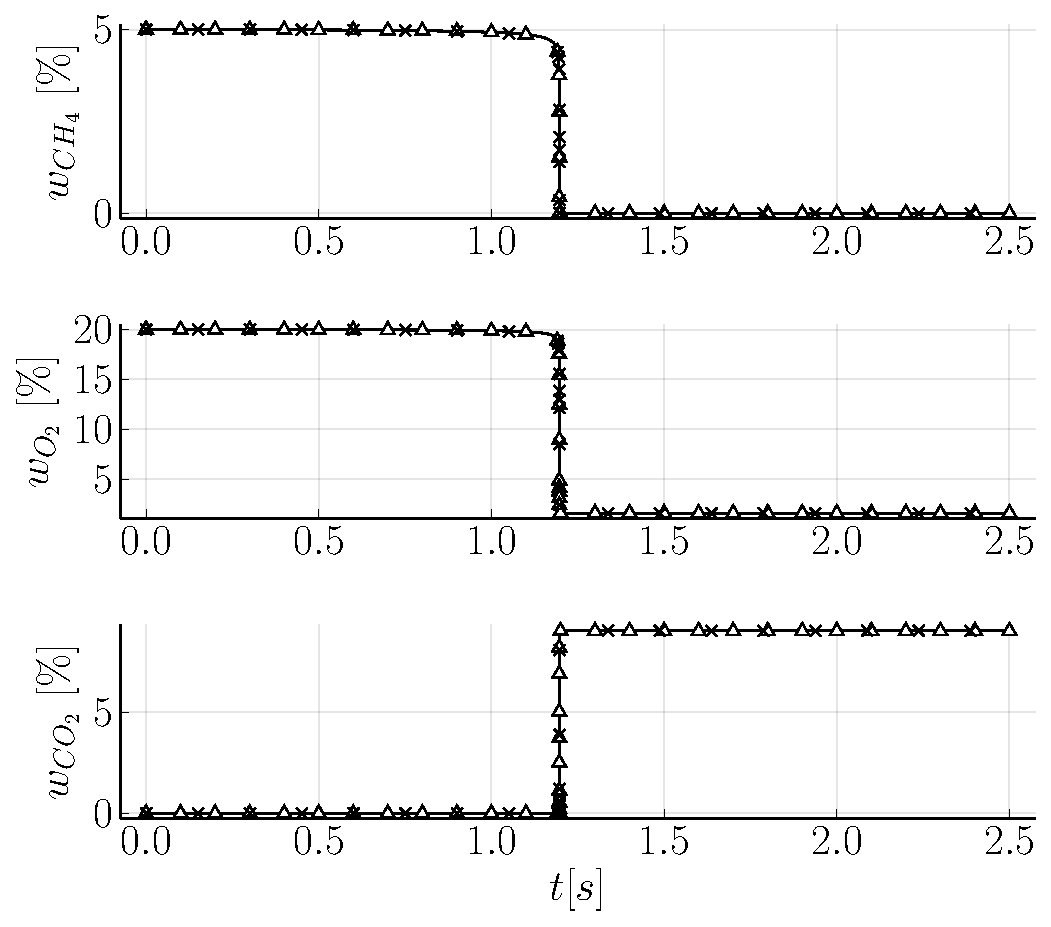
\includegraphics[width=0.5\textwidth]{figures/all validation.pdf}}
\caption{comparison between different species profiles obtained by different software .-----, AD tool; x, Cantera; $\Delta$, Flame Master}
    \label{fig:figure3}
\end{figure}
The validation of the sensitivity analysis is carried out using CSD, two different mechanisms with various environments are used for this purpose. Starting with the $h2vb$ mechanism as a preliminary step due to the small size of the mechanism and the huge importance of hydrogen fuel. Considering the following  initial mass fractions of $X_{H_2} = 0.09$ and $X_{O_2} = 0.18$ in $N_2$, as initial temperature 1000 K at atmospheric pressure condition is used for all of the $h2vb$ sensitivity results unless different composition is stated. Figure~\ref{fig:figure4} shows a good agreement between the results of {\color{red} name of the tool} and CSD.  The reaction  $H+O_2=>O+OH$ is the dominant reaction in the ignition process in terms of Arrihinieus parameters, showing the importance of the direct oxidation of $H_2$ on the gradients.
 
  {\color{red} discuss the same results for GRI}.
\begin{figure}
\centering
 {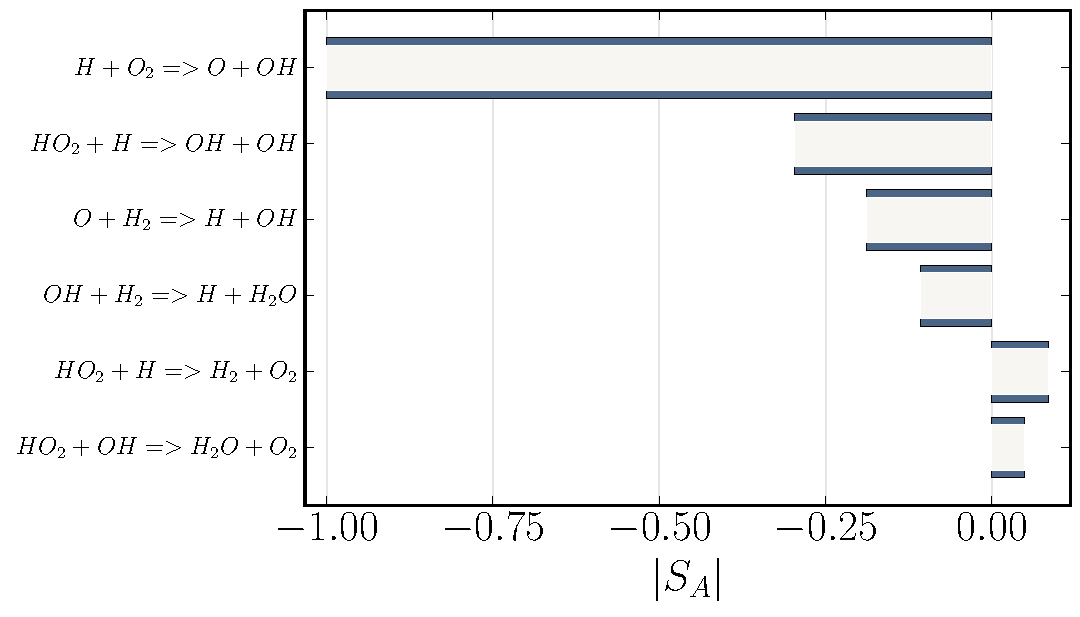
\includegraphics[width=0.5\textwidth]{figures/H2_SA_Validation.pdf}}
\caption{sensitivity analysis of ignition delay time with respect to $A$ for most dominant ten reactions}
    \label{fig:figure4}
\end{figure}

\begin{figure}
\centering
 {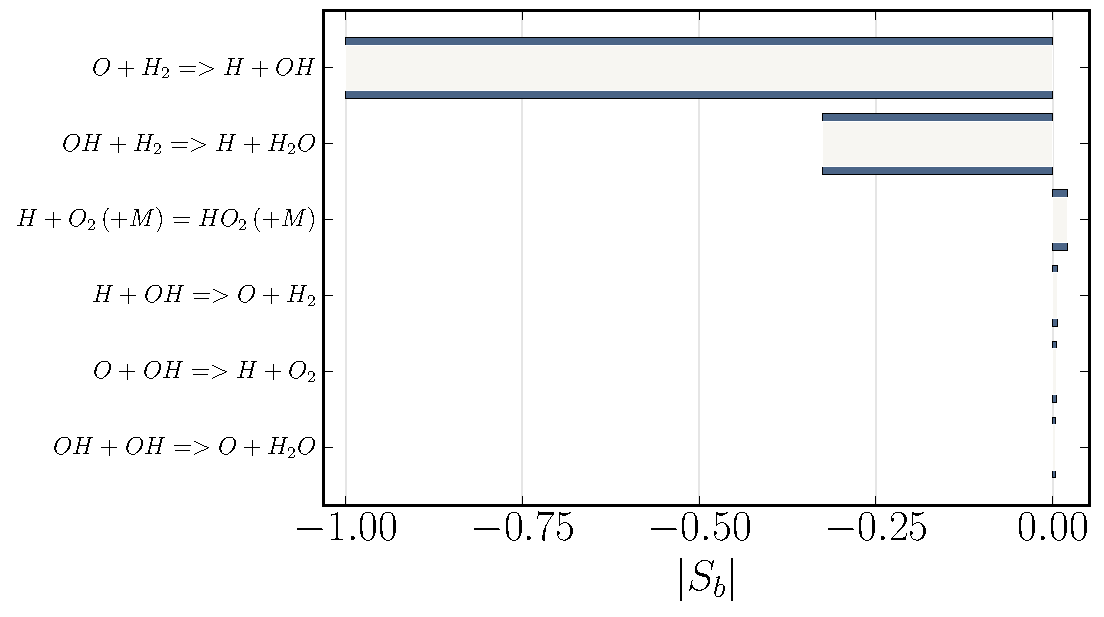
\includegraphics[width=0.5\textwidth]{figures/H2_Sb_Validation.pdf}}
\caption{sensitivity analysis of ignition delay time with respect to $\beta$ for most dominant ten reactions}
    \label{fig:figure5}
\end{figure}

\begin{figure}
\centering
 {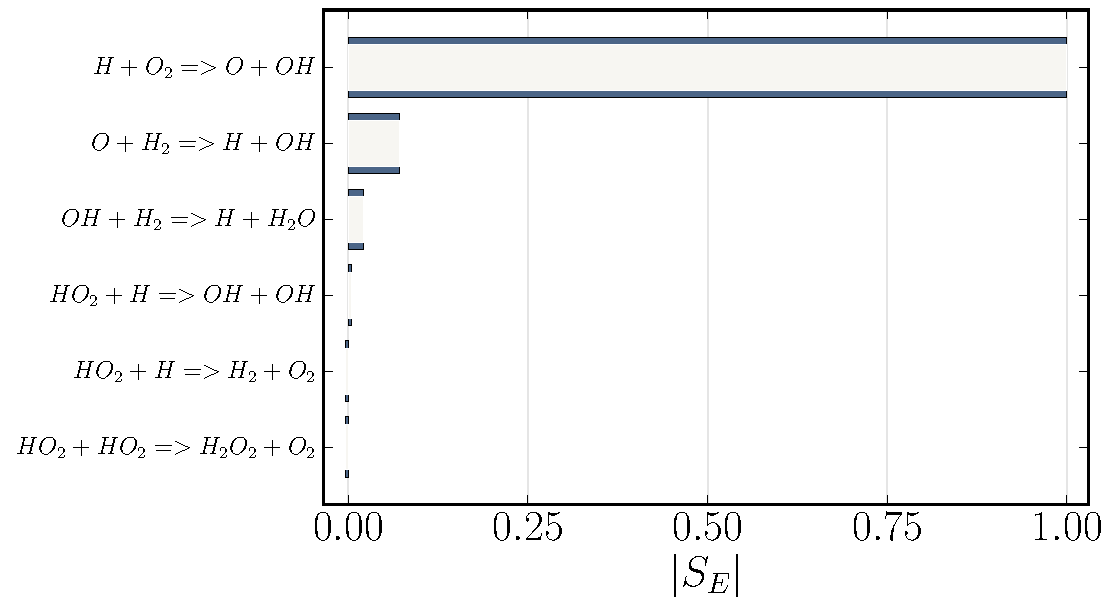
\includegraphics[width=0.5\textwidth]{figures/H2_SE_Validation.pdf}}
\caption{sensitivity analysis of ignition delay time with respect to $E$ for most dominant ten reactions}
    \label{fig:figure6}
\end{figure}

%
%
%\begin{figure}
%\centering
%\subfloat[Gas phase temperature]{\includegraphics[width=0.33\textwidth]{figures/fTemp-validation.pdf}\label{fig:figure3a}}
%\subfloat[$Y_{\mathrm{O}_2}$]{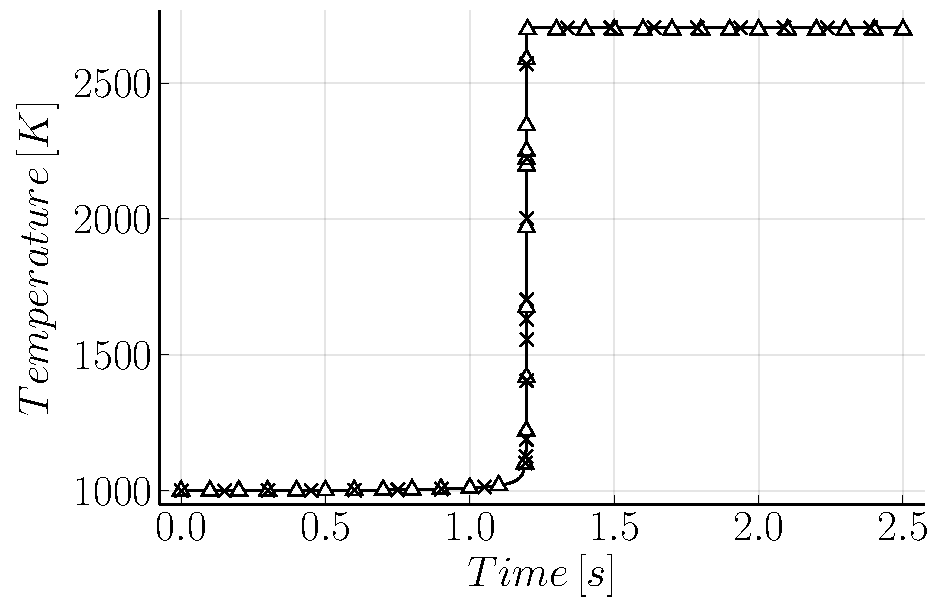
\includegraphics[width=0.33\textwidth]{figures/Temp-validation.pdf}\label{fig:figure3b}}
%\subfloat[$Y_{\mathrm{CO}_2}$]{
%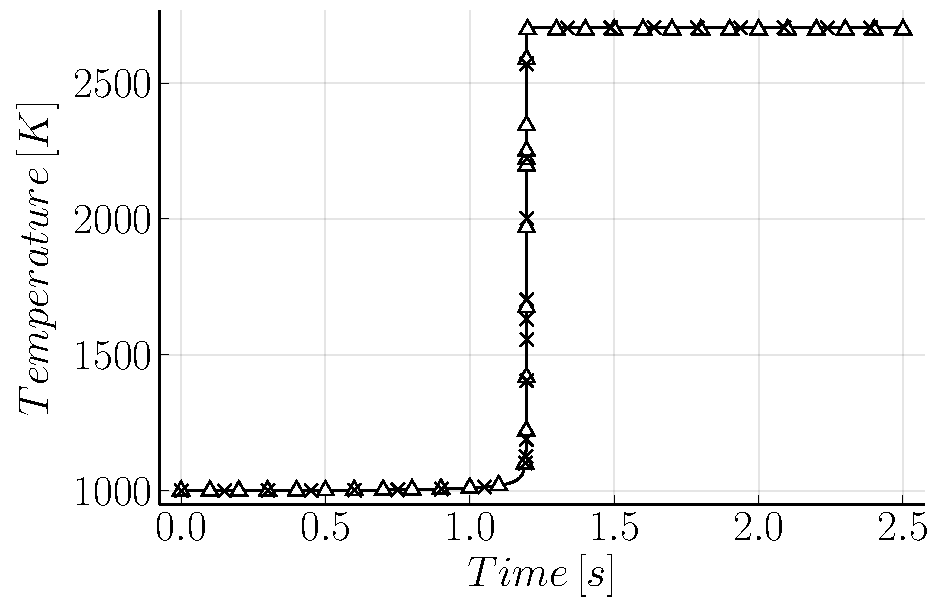
\includegraphics[width=0.33\textwidth]{figures/Temp-validation.pdf}\label{fig:figure3c}}
%\caption{TBD}
%\label{fig:figure3}
%\end{figure}
%The validation of the sensitivity analysis is carried out using CSD, two different mechanisms with various environments are used for this purpose. Starting with the $h2vb$ mechanism as a preliminary step due to the small size of the mechanism and the huge importance of hydrogen fuel. Considering the following  initial mass fractions of $X_{H_2} = 0.09$ and $X_{O_2} = 0.18$ in $N_2$, as initial temperature 1000 K at atmospheric pressure condition is used for all of the $h2vb$ sensitivity results unless different composition is stated. Figure~\ref{fig:figure4} shows a good agreement between the results of {\color{red} name of the tool} and CSD. the reaction  {\color{red} name of the reaction} is the dominant reaction in the ignition process in terms of Arrihinieus parameters. 
 

\subsection{Fall off and third body reactions parameter}
As mentioned, most of the IDT sensitivities studies in the literatures concentrate on the Arrihnius parameters only{\color{red} add ref} neglecting other reaction models, although, many different fuel mechanism contains third body and fall-off reactions{\color{red} add ref}. Considering the gradients of IDT with respect to enhanced third body efficiency $\alpha$ inform that for $h_2v1b$ scheme $\alpha_{N_2}$ that corresponds to the reaction $H+O_2 (+M)=> HO_2(+M)$as shown in figure~\ref{fig:figure9}. This result is traced back to the fact that$M_j=\sum_{}^{}\alpha_{i,j} [X_i]$  and $h_2v1b$ mechanism does not specify a certain values for $\alpha_{i,j}$, and $[X_{N_2}]$ is the supreme species so the value of $\alpha$ assigned to $N_2$ will have the maximum gradients.
 In case of GRI mechanism 
%all the species contribute equally so the major $\alpha_{i,j}$ is the one re $[X_i]$. Based on that,  
\begin{figure}
\centering
 {\includegraphics[width=0.5\textwidth]{figures/alpha.pdf}}
\caption{sensitivity with respect to thermodynamic coefficient $a_1$}
    \label{fig:figure9}
\end{figure}

\subsection{Thermodynamic parameters}
One of the important aspects when analysing the ignition process is not only the reactions behaviour but also, the effect of the thermodynamic quantities and it's impact on system sensitivities. However, it is not straightforward to extract the derivatives of any QoI with respect to NASA polynomial coefficients, but as AD provides a full accessibility to the gradients with respect to all system parameters, it is possible to provide a full analysis for the sensitivity with respect to Thermodynamic parameters. 
Figure~\ref{fig:figure10} 
shows that $a_{1:5_{N_2}}$ dominating the other species. This can be returned to the large value of $Y_{N_2}$, which mainly influences $C_v$ mixture average. As $N_2$ is an inert species in $h_2v$ scheme. However, $H_2O$  leads $a_6$ sensitivity, that inform the importance of $H_{H_2O}$ for IDT.


Moreover, $H_2O_2$ and $OH$ come at the top of $a_7$ gradients, this is associated to the key rule of  the two species entropy's' in IDT.

\begin{figure}
\centering
 {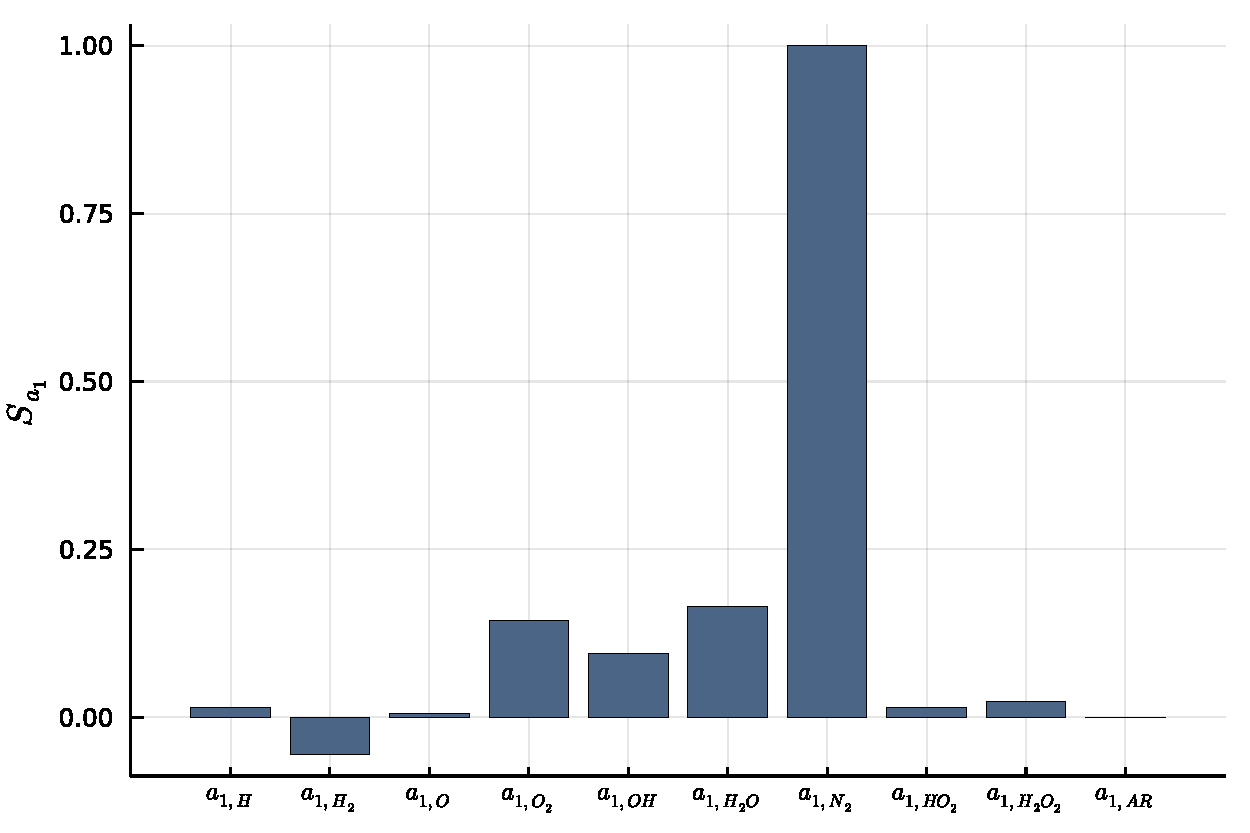
\includegraphics[width=0.5\textwidth]{figures/a1.pdf}}
\caption{sensitivity with respect to thermodynamic coefficient $a_1$}
    \label{fig:figure7}
\end{figure}

Extracting the sensitivities with respect to NASA Polynomial coefficients at high temperature provides a similar behaviour as in low $T$ as it is shown in figure ~\ref{fig:figure10} except for $ a_{7_{H_2O_2}}$ where the sign of the gradient is changed.
 which can be related to the increase in the value of $Y_{H_2O}$ due to the combustion process.

 This demonstrates that  thermodynamic properties for diluted mixture is controlled by the diluted species.  
 

\begin{figure}
\centering
 {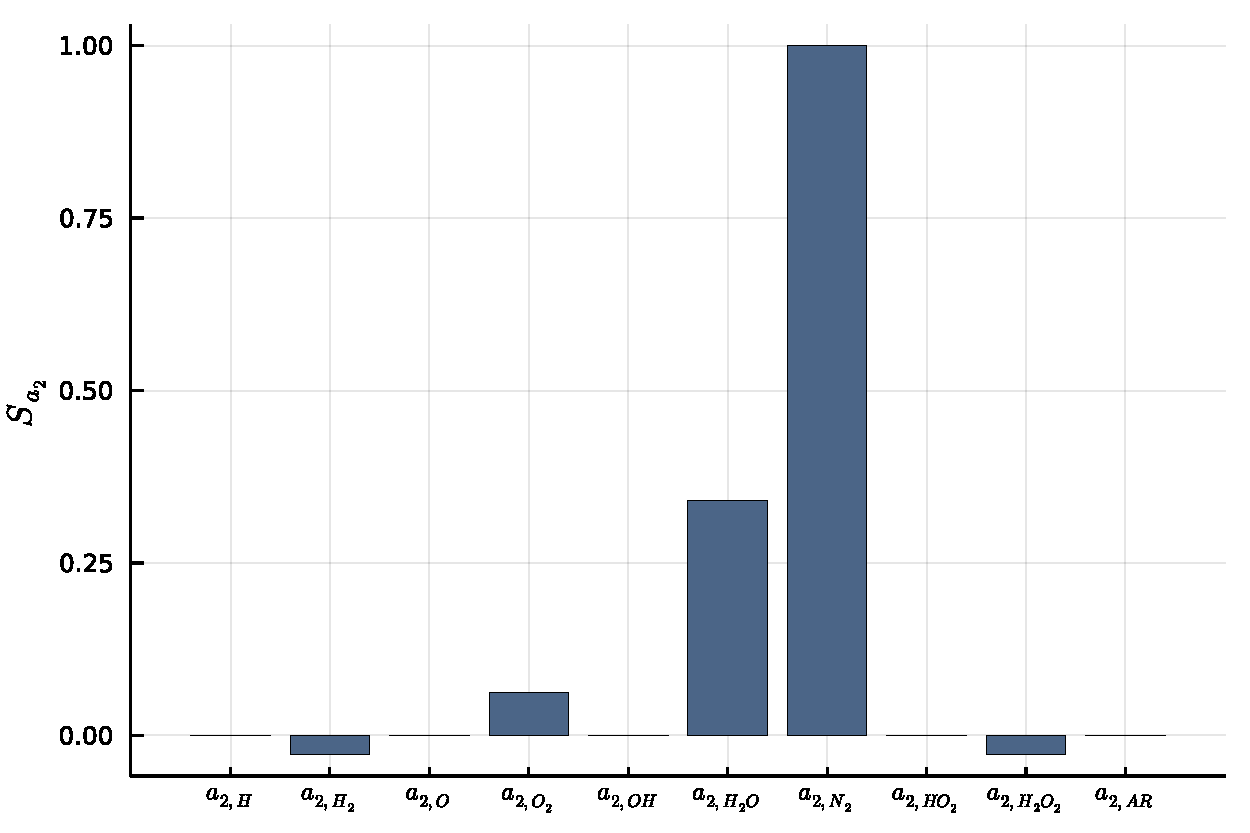
\includegraphics[width=0.5\textwidth]{figures/aa2.pdf}}
\caption{sensitivity with respect to thermodynamic coefficient $a_1$}
    \label{fig:figure8}
\end{figure}

\begin{figure}
\centering
 {\includegraphics[width=0.5\textwidth]{figures/thermodynamics.pdf}}
\caption{sensitivity with respect to thermodynamic coefficients}
    \label{fig:figure10}
\end{figure}
 {\color{red} discuss the same results for GRI}.
\subsection{Sensitivity evolution in time}

\subsection{Performance}
The main advantage of using {\color{red} Tool} is not only to get derivatives with accuracy equal to analytical ones through AD approach, but also, decreasing the computational time of creating the Jacobian using the traditional approaches. Table~\ref{table1} shows a comparison between the single step evaluation for the different Jacobians, which clearly proves the supremacy of   {\color{red} Tool}  performance comparing to other methods. 


The comparison is held for an instant instead of the whole time domain to avoid any effect could come from the time integrator with adaptive discritization as this is not the target of the discrimination. Further analysis for the {\color{red} Tool} can be found on {\color{red} add ref}.

\section{Conclusions}
\label{Conclusions}

TBD

\section*{Acknowledgments}
\label{Acknowledgments}

TBD 

%% References can be added with or without bibTeX database
%%
%% References with bibTeX database:
%% The bibliography style, elsarticle-num.bst, is used and available within the template package
\bibliography{references.bib} %%User-specified
\bibliographystyle{elsarticle-num-CNF.bst}

%% References without bibTeX database:
%%
% \begin{thebibliography}{99}
% \bibitem{Westbrook_1984} C. Westbrook, F. Dryer, Progress in Energy and Combustion Science 10 (1984) 1--57.
% \bibitem{Peters_2002} N. Peters, G. Paczko, R. Seiser, K. Seshadri, Combustion and Flame 128 (2002) 38--59.
% \end{thebibliography}

\end{document}

%%
%% End of file `template.tex'.
